Feature selection was performed in the exact same way as in case of noise-free images, meaning by a stepwise regression algorithm with five steps forward and three steps backwards. As a result of this process, from a set of 196 available features, 10 features were chosen. Figures \ref{fig:nonlinear_noised_features_colour} and \ref{fig:nonlinear_noised_features_percentage} depict which features were chosen for this experiment just like in case of the previous experiment. 
\begin{figure}[ht]
    \centering
    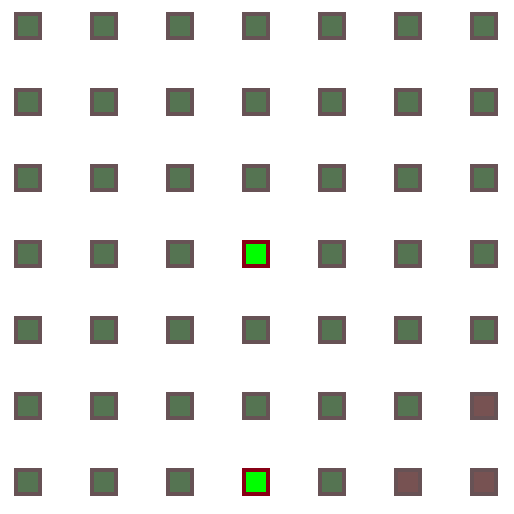
\includegraphics[width=0.52\textwidth]{nonlinear_noised/features/grid_colour_chosen_noised.png}
    \caption{Chosen grid colour features for experiments on noised data.}
    \label{fig:nonlinear_noised_features_colour}
\end{figure}
\begin{figure}[ht]
    \centering
    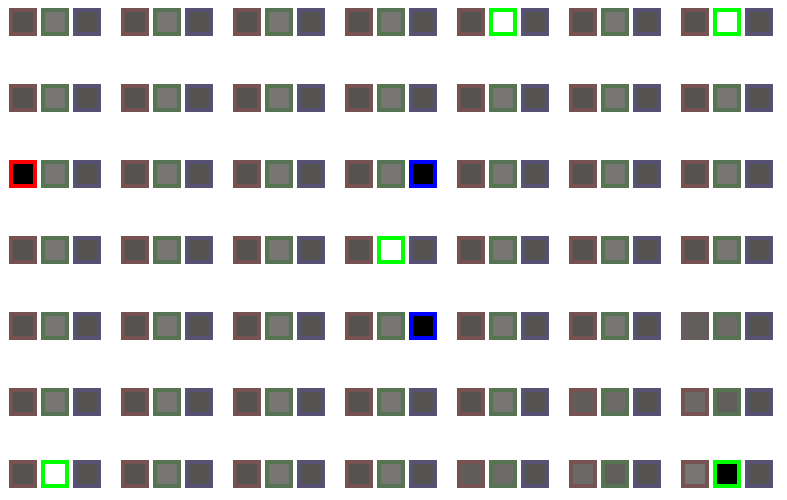
\includegraphics[width=\textwidth]{nonlinear_noised/features/grid_colour_percentage_chosen_noised.png}
    \caption{Chosen grid neighbour colour percentage features for experiments on noised data.}
    \label{fig:nonlinear_noised_features_percentage}
\end{figure}

When it comes to grid colour features only two were chosen, which is four less than in case of the optimal feature set for segmentation of noise-free images. However, the chosen two features, which are the colour of the superpixel under consideration, and the colour of a middle superpixel in the bottom row of the grid were also a part of a feature set used in the previous experiment. When it comes to features of neighbour colour percentages, two fewer features were chosen comparing to a noise-free case. Once again, a percentage of green neighbours of the superpixel under consideration is taken into account. There are also two other features of green neighbours percentage that were chosen for both, noise-free and noised data. 

In order to prove the importance of proper feature selection for semantic segmentation of noised data, figures \ref{fig:noised_fi1_all_features} and \ref{fig:noised_fi1_selected_features} were prepared. Both figures show probabilities $p(y|x)$ computed for each label in the same form as it was in the previous section about semantic segmentation of noise-free images. On these figures the same 3 test samples are shown, however, the first one presents the results if all 196 features were used, and the second one if a set of 10 selected features only. 

\begin{center}
    \renewcommand{\arraystretch}{4}
    \begin{tabular}{cccc}
        \textit{test image} &
        \fcolorbox{black}{white}{\includegraphics[align=c,width= 0.22\textwidth]{nonlinear_noised/fi1_all_features/1/image.png}} &
        \fcolorbox{black}{white}{\includegraphics[align=c,width= 0.22\textwidth]{nonlinear_noised/fi1_all_features/2/image.png}} &
        \fcolorbox{black}{white}{\includegraphics[align=c,width= 0.22\textwidth]{nonlinear_noised/fi1_all_features/3/image.png}}  \\
        \textit{label 0} &
        \fcolorbox{black}{white}{\includegraphics[align=c,width= 0.22\textwidth]{nonlinear_noised/fi1_all_features/1/label_0.png}} &
        \fcolorbox{black}{white}{\includegraphics[align=c,width= 0.22\textwidth]{nonlinear_noised/fi1_all_features/2/label_0.png}} &
        \fcolorbox{black}{white}{\includegraphics[align=c,width= 0.22\textwidth]{nonlinear_noised/fi1_all_features/3/label_0.png}} \\
        \textit{label 1} &
        \fcolorbox{black}{white}{\includegraphics[align=c,width= 0.22\textwidth]{nonlinear_noised/fi1_all_features/1/label_1.png}} &
        \fcolorbox{black}{white}{\includegraphics[align=c,width= 0.22\textwidth]{nonlinear_noised/fi1_all_features/2/label_1.png}} &
        \fcolorbox{black}{white}{\includegraphics[align=c,width= 0.22\textwidth]{nonlinear_noised/fi1_all_features/3/label_1.png}} \\
        \textit{label 2} &
        \fcolorbox{black}{white}{\includegraphics[align=c,width= 0.22\textwidth]{nonlinear_noised/fi1_all_features/1/label_2.png}} &
        \fcolorbox{black}{white}{\includegraphics[align=c,width= 0.22\textwidth]{nonlinear_noised/fi1_all_features/2/label_2.png}} &
        \fcolorbox{black}{white}{\includegraphics[align=c,width= 0.22\textwidth]{nonlinear_noised/fi1_all_features/3/label_2.png}} \\
        \textit{label 3} &
        \fcolorbox{black}{white}{\includegraphics[align=c,width= 0.22\textwidth]{nonlinear_noised/fi1_all_features/1/label_3.png}} &
        \fcolorbox{black}{white}{\includegraphics[align=c,width= 0.22\textwidth]{nonlinear_noised/fi1_all_features/2/label_3.png}} &
        \fcolorbox{black}{white}{\includegraphics[align=c,width= 0.22\textwidth]{nonlinear_noised/fi1_all_features/3/label_3.png}}
    \end{tabular}
    \captionof{figure}{Visual representation of conditional probabilities $p(y|x)$ for noised images without feature selection.}
    \label{fig:noised_fi1_all_features}
\end{center}


\begin{center}
 \renewcommand{\arraystretch}{4}
    \begin{tabular}{cccc}
        \textit{test image} &
        \fcolorbox{black}{white}{\includegraphics[align=c,width= 0.22\textwidth]{nonlinear_noised/fi1_selected_features/1/image.png}} &
        \fcolorbox{black}{white}{\includegraphics[align=c,width= 0.22\textwidth]{nonlinear_noised/fi1_selected_features/2/image.png}} &
        \fcolorbox{black}{white}{\includegraphics[align=c,width= 0.22\textwidth]{nonlinear_noised/fi1_selected_features/3/image.png}}  \\
        \textit{label 0} &
        \fcolorbox{black}{white}{\includegraphics[align=c,width= 0.22\textwidth]{nonlinear_noised/fi1_selected_features/1/label_0.png}} &
        \fcolorbox{black}{white}{\includegraphics[align=c,width= 0.22\textwidth]{nonlinear_noised/fi1_selected_features/2/label_0.png}} &
        \fcolorbox{black}{white}{\includegraphics[align=c,width= 0.22\textwidth]{nonlinear_noised/fi1_selected_features/3/label_0.png}} \\
        \textit{label 1} &
        \fcolorbox{black}{white}{\includegraphics[align=c,width= 0.22\textwidth]{nonlinear_noised/fi1_selected_features/1/label_1.png}} &
        \fcolorbox{black}{white}{\includegraphics[align=c,width= 0.22\textwidth]{nonlinear_noised/fi1_selected_features/2/label_1.png}} &
        \fcolorbox{black}{white}{\includegraphics[align=c,width= 0.22\textwidth]{nonlinear_noised/fi1_selected_features/3/label_1.png}} \\
        \textit{label 2} &
        \fcolorbox{black}{white}{\includegraphics[align=c,width= 0.22\textwidth]{nonlinear_noised/fi1_selected_features/1/label_2.png}} &
        \fcolorbox{black}{white}{\includegraphics[align=c,width= 0.22\textwidth]{nonlinear_noised/fi1_selected_features/2/label_2.png}} &
        \fcolorbox{black}{white}{\includegraphics[align=c,width= 0.22\textwidth]{nonlinear_noised/fi1_selected_features/3/label_2.png}} \\
        \textit{label 3} &
        \fcolorbox{black}{white}{\includegraphics[align=c,width= 0.22\textwidth]{nonlinear_noised/fi1_selected_features/1/label_3.png}} &
        \fcolorbox{black}{white}{\includegraphics[align=c,width= 0.22\textwidth]{nonlinear_noised/fi1_selected_features/2/label_3.png}} &
        \fcolorbox{black}{white}{\includegraphics[align=c,width= 0.22\textwidth]{nonlinear_noised/fi1_selected_features/3/label_3.png}}
    \end{tabular}
    \captionof{figure}{Visual representation of conditional probabilities $p(y|x)$ for noised images after feature selection.}
    \label{fig:noised_fi1_selected_features}
\end{center}

As visible, for the set of all features, labellings of individual superpixels based on the computed probabilities $p(y|x)$ are much worse. Though classes of the objects are generally recognised correctly, the classification of superpixels on the boundaries between differently coloured objects is quite poor. This is especially visible on regions with label 3, as the shape of a letter H is more complex than that of a circle or a square and as a result, more superpixels are incorrectly labelled. This happens even on test images that do not contain any noise. If an original image was not shown, then it would be hard to say in what shape those objects are. On the other hand, using only a limited set of 10 selected features the number of incorrectly labelled superpixels is much smaller. Individual objects are clearly distinguishable and even the shape of a letter H for regions with \nth{3} class is sustained.

What is more, thanks to the presence of contextual features in a feature function definition, the unary potential has denoising abilities. If there is only one noised superpixel surrounded by neighbours of the same colour, the effect of the noise on the final labelling is diminished. This is especially visible in the second test sample presented in Figure \ref{fig:noised_fi1_selected_features}. There are around 15 noised superpixels and for the majority of them the probability of the correct label is still close to 100\%. Usually, the difficulty lies in a proper labelling of noised superpixels which are close to the boundary between different objects. However, even if the most probable label chosen by the unary potential is not the expected one, there is also a pairwise potential which aim is to cope with noises in an image basing on the colour similarities between superpixels of the original image.

